\documentclass[10pt]{beamer}

\usepackage{xeCJK}
\setCJKmainfont{Noto Sans CJK JP}
\xeCJKsetup{PunctStyle=kaiming,CJKspace=true,CheckSingle=true} 

\usepackage{subfigure}
\usepackage{amssymb, amsmath, amsfonts,verbatim}
\usepackage{tikz}
\graphicspath{ {./} }
\usetikzlibrary{matrix,arrows,fit,backgrounds,mindmap,plotmarks,decorations.pathreplacing}
\usepackage{tkz-euclide}
\usetkzobj{all}
\usepackage{pgfplots}
\pgfplotsset{compat=1.12}
\pgfdeclarelayer{background}
\pgfsetlayers{background,main}

\tikzset{decoration={name=none},}

\newlength\figureheight
\newlength\figurewidth

\newcommand{\tikzdir}[1]{#1.tikz}
\newcommand{\inputtikz}[1]{\input{\tikzdir{#1}}}

\newcommand{\tI}{\tilde {\mathcal I}}
\newcommand{\tA}{\tilde A}
\newcommand{\ty}{\tilde y}
\newcommand{\tx}{\tilde x}
\newcommand{\tw}{\tilde w}
\newcommand{\tv}{\tilde v}
\newcommand{\tC}{\tilde C}
\newcommand{\tP}{\tilde P}
\newcommand{\Ic}{{\mathcal I^c}}
\newcommand{\J}{{\mathcal J}}
\newcommand{\K}{{\mathcal K}}

\DeclareMathOperator{\Smin}{Smin}
\DeclareMathOperator{\Smid}{Smid}
\DeclareMathOperator{\Smax}{Smax}
\DeclareMathOperator{\MSE}{MSE}
\DeclareMathOperator{\rank}{rank}
\DeclareMathOperator{\Med}{Med}
\DeclareMathOperator{\Max}{Max}
\DeclareMathOperator{\Min}{Min}
\DeclareMathOperator{\tr}{tr}
\DeclareMathOperator{\Cov}{Cov}
\DeclareMathOperator{\logdet}{log\;det}
\DeclareMathOperator{\argmin}{arg\;min}
\DeclareMathOperator{\argmax}{arg\;max}
\let\Tiny\tiny

\title[Secure CPS]{基于数据驱动的主动入侵检测}
\author[Yilin Mo]{莫一林}
\institute[Tsinghua]{
  清华大学 自动化系
}
\date[Nov 25, 2018]{ 人工智能与群体智能研讨会\\ 
  \small Joint Work with Hanxiao Liu, Jiaqi Yan and Karl H. Johansson}

\usetheme[subsectionpage=none,block=fill]{metropolis}
\definecolor{thupurple}{RGB}{102,8,116}
\definecolor{caltechcolor}{RGB}{102,8,116}
\setbeamercolor{title separator}{fg=black!50}
\setbeamercolor{frametitle}{bg=thupurple!70!black}
 

\begin{document}

\maketitle 

\section{信息物理系统安全研究简介}

\begin{frame}{Cyber-Physical System}
  \begin{itemize}
  \item Cyber-Physical Systems (CPSs) refer to the embedding of computation, communication and control into physical spaces.
    \begin{center}
      \begin{tikzpicture}[scale=0.45,transform shape,level distance=0cm,
        level 1 concept/.append style={sibling angle=120,minimum size = 3cm},
        ]
        \path [draw=thupurple!50,fill=thupurple!20,thick,rounded corners] (-10,-4.5) rectangle (10,7);
        \node at (-9,6) [anchor=north west] {\Huge 物理空间};
        \path[mindmap,concept color=black,text=white]
        node[concept] {\Huge CPS}
        [clockwise from=330]
        child[concept color=green!50!black] { node[concept](communication) {\huge 通讯} }
        child[concept color=red] { node[concept](control) {\huge 控制} }
        child[concept color=blue] { node[concept](computation) {\huge 计算} };
      \end{tikzpicture}
    \end{center}
  \item Applications: aerospace, chemical processes, civil infrastructure, energy, manufacturing and transportation. 
  \end{itemize}
\end{frame}

\begin{frame}{Security Threats for the CPS}
  \begin{itemize}
  \item The next generation CPS: Smart Grids, Smart Buildings, Smart Home, Internet of Things, will make extensive use of widespread sensing and networking.
  \item As the CPSs become ``smarter'', they are also more vulnerable to malicious attacks.
  \end{itemize}
  \begin{figure}[ht]
    \centering
    \includegraphics[width=0.6\textwidth]{SmartHome.jpg}
  \end{figure}
\end{frame}

\begin{frame}{Stuxnet}
  \begin{figure}[ht]
    \centering
    \includegraphics[width=0.8\textwidth]{stuxnet.jpg}
  \end{figure}
  Stuxnet is the first discovered malware that spies on and subverts industrial control systems. It was discovered in June 2010. 
\end{frame}

\begin{frame}{Industrial Control Systems}
  \begin{figure}[ht]
    \centering
    \includegraphics[width=0.6\textwidth]{cert.jpg}
  \end{figure}
 In FY 2014, ICS-CERT (Industrial Control Systems Cyber Emergency Response Team) received and responded to 245 incidents as reported by asset owners and industry partners. This number increased to 290 in FY 2016.
\end{frame}


\begin{frame}{Industrial Control Systems}
   The scope of incidents encompassed a vast range of threats and observed methods for attempting to gain access to both business and control systems infrastructure, including but not limited to the following:
  \begin{enumerate}
  \item  Unauthorized access and exploitation of Internet facing ICS/Supervisory Control and Data Acquisition (SCADA) devices,
  \item 	 Exploitation of zero-day vulnerabilities in control system devices and software, 
  \item  	 Malware infections within air-gapped control system networks,
  \item \dots
  \end{enumerate}

\end{frame}

\begin{frame}{Attack Through Compromised Supply Chain}
  \begin{figure}[ht]
    \centering
    \includegraphics[width=0.8\textwidth]{boeing.jpg}
    \caption{Boeing 787 outsourced 70\% of its parts.}
  \end{figure}
\end{frame}

\begin{frame}{2003 Northeast Blackout}
  \begin{figure}[<+htpb+>]
    \begin{center}
      \includegraphics[width=0.60\textwidth]{blackout.jpg}
      \caption{A successful attack on CPS can have devastating effects.}
    \end{center}
  \end{figure}
\end{frame}

\begin{frame}{How to deal with CPS security threats}
  \begin{exampleblock}{}
    {\it 知彼知己,百战不殆;不知彼而知己,一胜一负;不知彼不知己,每战必败}
    \vskip5mm
    \hspace*\fill{ \it\small--- 孙子兵法}
  \end{exampleblock}

  \begin{enumerate}
  \item Intrusion detection and isolation
  \item Resilient information fusion and control
  \end{enumerate}
\end{frame}

\section{重放攻击与物理水印}

\begin{frame}{Stuxnet}
  \begin{itemize}
    \item NY times:``The worm itself now appears to have included two major components. One was designed to send Iran's nuclear centrifuges spinning wildly out of control. Another seems right out of the movies: The computer program also \alert{secretly recorded what normal operations at the nuclear plant looked like, then played those readings back to plant operators}, like a pre-recorded security tape in a bank heist, so that it would appear that everything was operating normally while the centrifuges were actually tearing themselves apart.''
  \end{itemize}
\end{frame}

\begin{frame}{System Model}
  \begin{block}{System Description}
      \begin{displaymath}
	\begin{split}
	  x(k+1) &= Ax(k)  + Bu(k)+w(k),\\
	  y(k) &= C x(k) + v(k).
	\end{split}
      \end{displaymath}
    \end{block}
    \begin{itemize}
      \item $x(k) \in \mathbb R^n$ is the state vector.
      \item  $y(k) \in \mathbb R^m$ is the measurements from the sensors.
      \item  $u(k) \in \mathbb R^p$ is the control input.
      \item $w(k),v(k),x(0)$ are independent Gaussian random vectors, and $x(0) \sim \mathcal N(0,\;\Sigma)$, $w(k) \sim \mathcal N(0,\;Q)$ and $v(k) \sim \mathcal N(0,\;R)$ with $Q,R>0$.
      \item The system is assumed to be controllable and observable.
    \end{itemize}
  \end{frame}

  \begin{frame}{LQG Controller and Kalman filter}
    \begin{itemize}
      \item We assume that the system operator wants to minimize the following cost function:
	\begin{displaymath}
	  J = \lim_{T\rightarrow \infty}\min_{u(0),\ldots,u(T)}E\frac{1}{T}\left[\sum_{k=0}^{T-1} x(k)'Wx(k)+u(k)'Uu(k)\right],
	\end{displaymath}
	where $W, U$ are positive semidefinite matrices. 
      \item The optimal controller is a fixed gain controller, which takes the following form:
	\begin{displaymath}
	  u(k) =  L^*\hat x(k),
	\end{displaymath}
      \item The optimal estimator (Kalman filter) follows the following update equations:
	\begin{align*}
	  \hat x(k+1|k) &= A\hat x(k)+Bu(k),\\
	  \hat x(k+1) &= \hat x(k+1|k) + K^*\left[y(k+1) - C\hat x(k+1|k)\right],
	\end{align*}
    \end{itemize}
  \end{frame}

  \begin{frame}{$\chi^2$ Failure Detector}
    \begin{itemize}
      \item The residue $z(k)$ of the Kalman filter is defined as
	\begin{displaymath}
	  z(k) \triangleq y(k) - C\hat x(k|k-1),
	\end{displaymath} 
	which is i.i.d. Gaussian distributed with zero mean. 
      \item $\chi^2$ detector triggers an alarm based on the following event:
	\begin{displaymath}
	  g(k)=  z(k)^T\mathcal P^{-1}z(k)> threshold,
	\end{displaymath}
	where $\mathcal P$ is the covariance matrix of $z(j)$ and $\mathcal T$ is the window size.
      \item The alarm rate at time $k$ is 
	\begin{displaymath}
	  \beta(k) = P(g(k) > threshold).
	\end{displaymath}
	If the system is operating normally, then the alarm rate is a constant, which we denote as the false alarm rate $\alpha$.
    \end{itemize}
  \end{frame}

  \begin{frame}{System Diagram}
    \begin{figure}[htpb]
      \begin{center}
	\inputtikz{systemdiagram}
      \end{center}
    \end{figure}
  \end{frame}

  \begin{frame}{Replay Attack Model}
    \begin{enumerate}
      \item The attacker can read and modify all the measurements $y(k)$ arbitrarily.
      \item It can inject an external control input $u^a(k)$ into the system. 
    \end{enumerate}
    The strategy of the attacker can be divided into two stages:
    \begin{enumerate}
      \item The attacker records a sufficient number of $y(k)$s without injecting any control input $u^a(k)$. 
      \item The attacker injects a sequence of desired control input $u^a(k)$ while replaying the previous recorded $y(k)$s starting from time $0$.
    \end{enumerate}
    When the system is under attack, the controller will be unable to perform closed-loop control. Hence the only way to counter this attack is to detect its presence. 
  \end{frame}

  \begin{frame}{Replay Attack: First Stage}
    \begin{figure}[htpb]
      \begin{center}
	\inputtikz{replaydiagramone}
      \end{center}
    \end{figure}
  \end{frame}

  \begin{frame}{Replay Attack: Second Stage}
    \begin{figure}[htpb]
      \begin{center}
	\inputtikz{replaydiagramtwo}
      \end{center}
    \end{figure}
  \end{frame}

  \begin{frame}{Feasibility of Replay Attacks}
    \begin{figure}[htpb]
      \setlength\figureheight{4.5cm}
      \setlength\figurewidth{10cm}
      \begin{center}
	\inputtikz{replayunstableA2}
      \end{center}
    \end{figure}
    Replay attack is not always feasible!
  \end{frame}

  \begin{frame}{Feasibility of Replay Attacks}
    \begin{figure}[htpb]
      \begin{center}
	\inputtikz{replaydiagramthree}
      \end{center}
    \end{figure}
  \end{frame}

  \begin{frame}{Feasibility of Replay Attacks}
    The update equation of Kalman filter follows:
    \begin{align*}
      \hat{x}(k+1|k)&=A\hat{x}(k)+Bu(k)=\left(A+BL^*\right)\hat{x}(k)\\
      &=\left(A+BL^*\right)\left(I-K^*C\right)\hat{x}(k|k-1)+\left(A+BL^*\right)K^*y(k).
    \end{align*}

    \begin{theorem}
      If $\mathcal A = (A+BL^*)(I-K^*C)$ is stable, then the detection rate of $\chi^2$ detector $\beta^c(k)$ converges to the false alarm rate $\alpha$ during the attack, i.e.,
      \begin{displaymath}
	\lim_{k\rightarrow\infty}\beta^c(k) = \alpha.  
      \end{displaymath}
      On the other hand, if $\mathcal A$ is strictly unstable, then the detection rate $\beta^c(k)$ converges to $1$, i.e.,
      \begin{displaymath}
	\lim_{k\rightarrow\infty}\beta^c(k) = 1.  
      \end{displaymath}
    \end{theorem}
  \end{frame}

  \begin{frame}{Countermeasures: Authentication and Watermarking}
    \begin{itemize}
      \item Challenge-response authentication is widely in cyber security, where one party presents a question ("challenge") and another party must provide a valid answer ("response") to be authenticated.
      \item Similarly, we could change the control law by adding a random watermarking signal:
	\begin{displaymath}
	  u(k) = L^*\hat x(k) + \zeta(k).
	\end{displaymath}
      \item The watermarking signal $\zeta(k)$ acts as a ``challenge'' and the sensor measurement is the ``response''. 
      \item During normal operation, the ``challenge'' and ``response'' are correlated through the system dynamics, while the correlation cease to exist when the replay begins.
      \item The CPS will remain stable. However, we sacrifice LQG performance since the control is not optimal.
    \end{itemize}
  \end{frame}

\begin{frame}{System with Physical Watermarks}
    \begin{figure}[htpb]
      \begin{center}
	\inputtikz{replaywithphywatermark}
      \end{center}
    \end{figure}
\end{frame}

\begin{frame}{Active Detection of Replay Attack}
  \setlength{\figureheight}{6cm}
  \setlength{\figurewidth}{7cm}
    \begin{figure}[htpb]
      \begin{center}
	\inputtikz{replay1}
      \end{center}
    \end{figure}
\end{frame}

\begin{frame}{Some Known Results}
  \begin{itemize}
  \item Assuming the watermarking signal is i.i.d. zero mean Gaussian with covariance $U$.
  \item The optimal watermarking signal design problem can be written as
    \begin{align*}
      &\mathop{\textrm{maximize}}\limits_{U}&
      & Detection\;Performance\\
      &\textrm{subject to}&
      & Additional\;LQG\;Cost \leq \delta \\
      &&& U \text{ is positive semidefinite.}
    \end{align*}
  \item The above problem can be relaxed into an Semi-Definite Programming problem. The optimal solution can be derived analytically using generalized eigenvectors.
  \item Also there are results on how to find the optimal \textbf{stationary} zero mean Gaussian watermarking signal.
  \item What if the system is \textbf{unknown}?
  \end{itemize}
\end{frame}

\section{主动检测机制的在线学习}

\begin{frame}{System Diagram}
  \begin{figure}[htpb]
    \inputtikz{systemdiagram2}
  \end{figure}
\end{frame}

\begin{frame}{Modified System Model}
  \begin{figure}
    \centering
    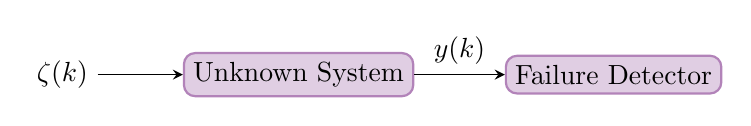
\begin{tikzpicture}
      \node (p1) at (0,0) {$\zeta(k)$};
      \node [draw=thupurple!50,fill=thupurple!20,thick,rounded corners] (p2) at (3,0) {Unknown System};
      \node [draw=thupurple!50,fill=thupurple!20,thick,rounded corners] (p3) at (7,0) {Failure Detector};
      \draw [semithick,-stealth] (p1)--(p2);
      \draw [semithick,-stealth] (p2)--node[above]{$y(k)$} (p3);
    \end{tikzpicture}
  \end{figure}
  \begin{enumerate}
  \item System Dynamics:
  \begin{align*}
    x(k+1) = A x(k) + B\zeta(k)+w(k), \;y(k)  &= C x(k) + v(k) . 
  \end{align*}
  \item LQG cost:
	\begin{align*}
		J = \lim_{T \to +\infty} \mathbb E\left [\frac{1}{T}\sum_{k=0}^{T-1} \begin{bmatrix}
		y(k)\\
		\zeta(k)
		\end{bmatrix}^TX \begin{bmatrix}
		y(k)\\
		\zeta(k)
		\end{bmatrix} \right ],
	\end{align*}
  \end{enumerate}
\end{frame}

\begin{frame}{Assumptions}
  \begin{itemize}
  \item The system is stable (or has been stabilized by some inner-loop controller), controllable and observable.
  \item $A$ has distinct eigenvalues.
  \item We can observe $y(k)$, and we know the dimension of the $x(k)$.
  \item The LQG weight matrix $X$ is known.
  \item The noise are all zero mean i.i.d. Gaussian.
  \end{itemize}
  \textbf{No additional knowledge} on the $A,B,C$ matrices or the covariance of the noise is assumed.
\end{frame}

\begin{frame}{Impact on the Control Performance}
  The additional LQG cost incurred by the watermarking signal is a linear function of $U$.
  \begin{displaymath}
    \text{Additional LQG cost} = \tr(U\mathcal X).
  \end{displaymath}
  where $\mathcal X$ is given by:
  \begin{align*}
  \mathcal X &\triangleq \sum_{k=0}^\infty\textcolor{thupurple}{\left(CA^kB\right)^T} X_{yy}\textcolor{thupurple}{\left(CA^kB\right)}+ \textcolor{thupurple}{\left(CB\right)^T}X_{y\phi} + X_{\phi y}\textcolor{thupurple}{CB}+ X_{\phi \phi}\\
  &= \sum_{k=0}^\infty \textcolor{thupurple}{H_k^T} X_{yy}\textcolor{thupurple}{H_k}+ \textcolor{thupurple}{H_0^T}X_{y\phi} + X_{\phi y}\textcolor{thupurple}{H_0}+ X_{\phi \phi}.
  \end{align*}
\end{frame}


\begin{frame}{Detecting Replay Attacks}
  \begin{itemize}
  \item In the absence of the attack:  
    \begin{align*} 
      y(k) &=\textcolor{red}{\boxed{\sum_{t=0}^{k-1} CA^{t}B  \zeta(k-1-t)}} + \textcolor{blue}{\boxed{\sum_{t=0}^{k-1}  CA^{t} w(k-1-t)+v(k) }}\\ 
            &=\textcolor{red}{\gamma(k-1)} +\textcolor{blue} {\vartheta(k-1)},
    \end{align*}
  \item  In the presence of the attack:
    \begin{align*}
      y^c(k) = y(k-\Delta k) = \textcolor{red}{\gamma(k-1-\Delta k)} + \textcolor{blue}{\vartheta(k-1-\Delta k)}.
    \end{align*}
  \item The KL divergence between ``compromised'' measurement $y^c(k)$ and ``normal'' measurement $y(k)$ is a convex function $U$, which satisfies
    \begin{displaymath}
      \frac{1}{2}\tr(U\mathcal P) \leq D_{KL}(y^c(k)||y(k))\leq \tr(U\mathcal P)-\frac{1}{2}\log(1+\tr(U\mathcal P)).
    \end{displaymath}
    Both the upper and lower bounds are increasing functions of $\tr(U\mathcal P)$, where
    \begin{align*}
    \mathcal P \triangleq\sum_{k=0}^\infty \textcolor{thupurple}{H_k^T\mathcal W^{-1}H_k},\\
    \end{align*}
    where $\mathcal W$ is the covariance of $\vartheta_{k-1}$.
  \end{itemize}
\end{frame}

\begin{frame}{Optimal Watermark}
  \begin{block}{Problem 1}
    \begin{align*}
      &\mathop{\textrm{maximize}}\limits_{U}&
      & \tr (U\textcolor{thupurple}{\mathcal P})\\
      &\textrm{subject to}&
      & \tr (U\textcolor{thupurple}{\mathcal X}) \leq \delta \\
      &&& U \text{ is positive semidefinite.}
    \end{align*}
  \end{block}
  \centering
  \begin{tikzpicture}
    \tkzDefPoint[label=-135:\scriptsize$O$](0,0){O}
    \tkzDefPoint(15:3){A}
    \tkzDefPoint(60:3){B}
    \tkzDefShiftPoint[B](10:1){B1}
    \tkzDefShiftPoint[B](190:1){B2}
    \tkzDefPoint[label=\scriptsize PSD-cone](37.5:3.5){C}
    \tkzFillPolygon[color=thupurple!20](A,B,O)
    \tkzDrawPoints[color=thupurple!50](B)
    \tkzDrawLines[color=thupurple!50,add=0 and 0.2](O,A O,B)
    \tkzDrawLines[color=thupurple!50](A,B)
    \tkzLabelSegments[pos=1.2,below](B,A){\scriptsize$\tr(U\mathcal X)=\delta$}
    \foreach \i in {-0.5,0,...,1.5}{
      \tkzDefShiftPoint[B1](-80:\i){b1}
      \tkzDefShiftPoint[B2](-80:\i){b2}
      \tkzDrawLines[color=black!50,dashed,add 0.5 and 0.5](b1,b2)
    }
  \end{tikzpicture}

  The optimal $U = \alpha vv^T$ is a rank-$1$ matrix. 
\end{frame}

\begin{frame}{Online-Watermark Design: Watermark Generation}
  \begin{figure}[t]
    \centering
    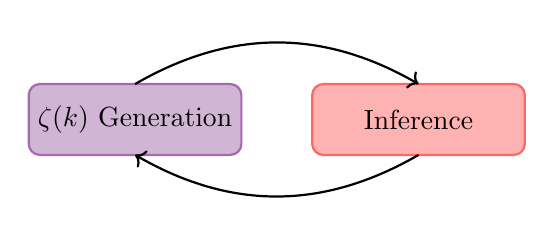
\begin{tikzpicture}[scale=0.9]
      \draw[thick,rounded corners,fill=thupurple!30,draw=thupurple!60] (0,1) rectangle (3,2);
      \node at (1.5,1.5) {$\zeta(k)$ Generation};
      \draw[thick,rounded corners,fill=red!30,draw=red!60] (4,1) rectangle (7,2);
      \node at (5.5,1.5) {Inference};
      \draw[thick,->] (1.5,2) to [bend left] (5.5,2);
      \draw[thick,->] (5.5,1) to [bend left] (1.5,1);
    \end{tikzpicture}
  \end{figure}
  \begin{itemize}
  \item Generate the ``optimal'' $U$: 
    \begin{align*}
      \hat U_k=&\mathop{\textrm{argmax}}\limits_{U}&
      & \tr (U\textcolor{thupurple}{\hat  P_k})\\
               &\textrm{subject to}&
      & \tr (U\textcolor{thupurple}{\hat  X_k}) \leq \delta \\
               &&& U \text{ is positive semidefinite.}
    \end{align*}
  \item     Generate the watermark signal:
    \begin{align*}
      \zeta(k) = \hat U_k^{1/2} \phi(k),\,where\; \phi(k)\sim\mathcal N(0,I).
    \end{align*}
  \end{itemize}
\end{frame}

\begin{frame}{Online-Watermark Design: Inference}
  \begin{figure}[t]
    \centering
    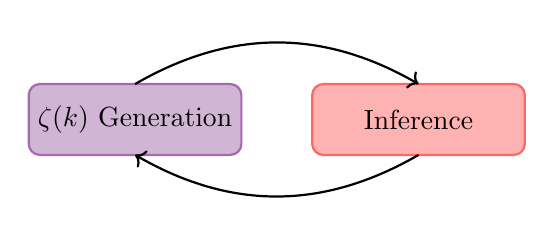
\begin{tikzpicture}[scale=0.9]
      \draw[thick,rounded corners,fill=thupurple!30,draw=thupurple!60] (0,1) rectangle (3,2);
      \node at (1.5,1.5) {$\zeta(k)$ Generation};
      \draw[thick,rounded corners,fill=red!30,draw=red!60] (4,1) rectangle (7,2);
      \node at (5.5,1.5) {Inference};
      \draw[thick,->] (1.5,2) to [bend left] (5.5,2);
      \draw[thick,->] (5.5,1) to [bend left] (1.5,1);
    \end{tikzpicture}
  \end{figure}
  \begin{itemize}
  \item If we compute $y(k)\phi(k)^T$, we get
    \begin{align*}
      y(k+1)\phi(k)^T &= \textcolor{thupurple}{CBU_k^{1/2}\phi(k)\phi(k)^T}+ \sum_{t=1}^{k}H_t U_{k-t}^{1/2} \phi(k-t) \phi(k)^T \\
                      &+\sum_{t=0}^{k}  CA^{t} w(k-t)\phi(k)^T +v(k+1)\phi(k)^T.
    \end{align*}
  \item One tentative way to infer $H_0$: 
    \begin{align*}
      H_0 \approx \text{the average of }y(k+1)\phi(k)^TU_{k}^{-1/2} . 
    \end{align*}
  \item Similarly we can estimate all $H_t$, and further infer $\mathcal P$ and $\mathcal X$.
  \end{itemize} 
\end{frame}

\begin{frame}{Key Problems with the Naive Approach}
  \begin{itemize}
  \item There are infinitely $H_t$s we need to infer
  \item The ``optimal'' $U_k$ is rank 1 and not invertible
  \end{itemize}
\end{frame}
\begin{frame}{Infer all $H_t$ using finitely many $H_t$s}
  \begin{itemize}
  \item We can only store \textbf{finitely many} $H_t=CA^tB$s, but we need \textbf{all} $H_t$ to compute $\mathcal P$ and $\mathcal X$.
  \item Solution: Cayley-Hamilton Theorem: 
    \begin{align*}
      p(A) = A^n + \alpha_{n-1}A^{n-1}+\ldots+\alpha_1 A + \alpha_0 I = 0     
    \end{align*}
    where $p(x)$ is the characteristic polynomial of $A$. 
  \item We can compute $A^n$ as
    \begin{align*}
      A^n =- \alpha_{n-1}A^{n-1}-\ldots-\alpha_1 A - \alpha_0 I.
    \end{align*}
  \item Similarly, we have
    \begin{align*}
      CA^nB =- \alpha_{n-1}CA^{n-1}B-\ldots-\alpha_1 CAB - \alpha_0 CB.
    \end{align*}
  \item As long as we know the characteristic polynomial of $A$, we can infer all $H_t$ from $H_0,\ldots, H_{n-1}$.
  \end{itemize} 
\end{frame}

\begin{frame}{Infer the Characteristic Polynomial}
  \begin{itemize}
  \item Since the system is controllable and observable, $p(A) = 0$ is equivalent to:
    \begin{align*}
      \begin{bmatrix}
        C\\
        CA\\
        \cdots\\
        CA^{n-1}
      \end{bmatrix}p(A)\begin{bmatrix}
        B&AB&\cdots&A^{n-1}B
      \end{bmatrix}=0.
    \end{align*}
  \item The above equation is equivalent to
    \begin{align*}
      \mathcal H   \begin{bmatrix}
        \alpha_0I\\
        \cdots\\
        \alpha_{n-1}I
      \end{bmatrix} + \begin{bmatrix}
        H_n\\
        \cdots\\
        H_{3n-2} 
      \end{bmatrix} = 0    ,
    \end{align*}
    where $\mathcal H$ is the Hankel matrix
    \begin{align*}
      \mathcal H \triangleq \begin{bmatrix}
        H_{0} & H_{1} &\cdots & H_{n-1}\\
        H_{1} & H_{2} &\cdots & H_{n}\\
        \vdots & \vdots &\ddots & \vdots \\
        H_{2n-2} & H_{2n-1} &\cdots & H_{3n-3}\\
      \end{bmatrix}. 
    \end{align*}
  \end{itemize} 
\end{frame}

\begin{frame}{Balance Exploration and Exploitation}
  \begin{itemize}
  \item Recall the structure of the optimal $U$ is $U = \alpha v v^T$.
  \item The optimal watermark will input the signal to the most ``informative'' direction $v$: Pure \textcolor{red}{Exploitation}.
  \item We could also consider classical system identification techniques, which use $U=I$: Pure \textcolor{blue}{Exploration}.
  \item To achieve a balance, choose
    \begin{align*}
      \hat U_k = \text{``optimal'' } U + k^{-\beta} I.
    \end{align*}
  \item More \textcolor{blue}{exploration} at the beginning and more \textcolor{red}{exploitation} towards the end.
  \end{itemize}
  \begin{theorem}
    Assume that $0 < \beta <1$, then we have $\hat U_k$ converges to the optimal $U$ a.s.
    
  \end{theorem}
\end{frame}



\begin{frame}{Tennessee Eastman Process}
  Here, we apply the proposed technique to the Tennessee Eastman Process (TEP).\\~\\
  \begin{itemize}
  \item The TEP is created to provide a realistic industrial process for developing studying and evaluating process control technology. 
  \item The Tennessee Eastman (TE) problem requires coordination of three unit operations: an exothermic, two-phase reactor, a flash separator and a reboiled  stripper.
  \item There are 41 measured output variables (with added measurement noise) and 12 manipulated variables.
  \item The original TE problem is very complex and the accurate model equations are not given by Eastman Chemical Company.   
  \end{itemize}
\end{frame}

\begin{frame}{Simplified TEP Model}
  Ricker (1993) proposed the following simplified TEP. The total volume is fixed. The reaction in the vapor phase is: $A+C\rightarrow D$.
  \begin{columns}
    \begin{column}{0.45\textwidth}
      \begin{figure}
        \includegraphics[width=0.9\textwidth]{simplifiedmodel.png}
        \caption{The simplified process}
      \end{figure}
    \end{column}
    \begin{column}{0.55\textwidth} 		
      \begin{itemize}
      \item The vessel: a combination of the reactor and separation system in the original TE Process;
      \item Feed 1: A, C and trace amounts of an inert B;
      \item Feed 2: pure A;
      \item Stream 3: purge rate;
      \item Stream 4: product rate;
      \item Vapor: A, B, C;\\
        Liquid: D.
      \end{itemize}
    \end{column}
  \end{columns}
\end{frame}

\begin{frame}{Simplified TEP Model}
  Ricker (1993) also provided a LTI dynamic model of the plant, and a corresponding robust controller with 4 outputs and 4 inputs.
  \begin{block}{Simplified transfer-function model}
    \begin{align*}
      \textbf{y}= \begin{bmatrix}
        F_4\\ 
        P\\ 
        y_{A3}\\
        V_L 
      \end{bmatrix}=\textbf{G}\textbf{u}=\begin{bmatrix}
        g_{11} & 0 & 0 & g_{14}\\ 
        g_{21} & 0 & g_{23} & 0\\ 
        0 & g_{32} & 0 & 0\\ 
        0 & 0 & 0 & g_{44} 
      \end{bmatrix}\begin{bmatrix}
        u_1\\ 
        u_2\\ 
        u_3\\ 
        u_4
      \end{bmatrix}
    \end{align*}
    For this model:\\
    \begin{itemize}
    \item Four manipulated variables: changes of the $i$th valve position.
    \item Four output variables: $F_4$: production rate, $P$: pressure,\\ $y_{A3}$: amount of A in purge, $V_L$: liquid inventory. 
    \item The individual transfer functions: $g_{11},\, g_{14},\, g_{21},\, g_{32},\, g_{44}$ and $g_{23}$ are also given. 
    \end{itemize}
  \end{block}
\end{frame}

\begin{frame}{Simulation Results}
  We apply the proposed technique to the simplified version of TE Process. \\~\\

  Discretizing the simplified TEP model with sampling period $T_{sp} = 0.6s$, we can derive the system matrices $A$, $B$ and $C$, where  
  \begin{itemize}
  \item $A$, $B$ and $C$ are sparse matrices.
  \item The eigenvalues of A is 0.9418,  0.9418, 0.5488, 0.5488, 0.4493, 0.0907, 0.0025. 
  \end{itemize}
  ~\\
  This system simulates a MIMO system with order $n = 7$ with  $p = 4$ inputs and $m = 4$ outputs. Moreover, the covariance matrices $Q = I_{7}$ and $ R = I_{4}$, $X = I_{8}$,  $\delta = 15$ ($13.13\%$ of the LQG cost $J = 114.22$), $\beta = \frac{1}{3}$.
\end{frame}

\begin{frame}
  \frametitle{The Watermark Signal Design}
  \begin{columns}
    \begin{column}{0.6\textwidth}
      \begin{figure}[h!]
         \inputtikz{errU1_te}
      \end{figure}
    \end{column}
    \begin{column}{0.4\textwidth}
      \begin{itemize}
      \item $U$: the optimal covariance of the watermark signal;
      \item $U_k$: the estimation of $U$.
      \end{itemize}
    \end{column}
  \end{columns}
  ~\\
  As time $k$ goes to infinity, $U_k$ converges to the optimal covariance of the watermark signal, $U$.
\end{frame}

\begin{frame}
  \frametitle{The detection performance}
  \begin{itemize}
  \item $g_n$: the output of the failure detector designed with know parameters
  \item $g$: the output of the failure detector when the parameters of the system are inferred through the learning technique. 
  \end{itemize}
  \begin{figure}[h!]
    \centering
     \inputtikz{gng_te}
  \end{figure}
\end{frame}

\section{结论}

\begin{frame}{Conclusion}
  We consider the impact of replay attacks on a steady state control system and propose watermarking scheme to actively detect the presence of replay attack. For systems whose parameters are unknown, we design learning based mechanism to identify the parameters and design the watermarking signals simultaneously.
\end{frame}

\begin{frame}[standout]
  感谢各位老师同学聆听,请大家批评指正!
\end{frame}

\end{document}

%%% Local Variables: 
%%% coding: utf-8
%%% mode: latex
%%% TeX-engine: xetex
%%% End: 